%; whizzy paragraph -pdf xpdf -latex ./whizzypdfptex.sh
%; whizzy-paragraph "^\\\\begin{frame}\\|\\\\emtext"
% latex beamer presentation.
% platex, latex-beamer でコンパイルすることを想定。 

%     Tokyo Debian Meeting resources
%     Copyright (C) 2012 Junichi Uekawa

%     This program is free software; you can redistribute it and/or modify
%     it under the terms of the GNU General Public License as published by
%     the Free Software Foundation; either version 2 of the License, or
%     (at your option) any later version.

%     This program is distributed in the hope that it will be useful,
%     but WITHOUT ANY WARRANTY; without even the implied warreanty of
%     MERCHANTABILITY or FITNESS FOR A PARTICULAR PURPOSE.  See the
%     GNU General Public License for more details.

%     You should have received a copy of the GNU General Public License
%     along with this program; if not, write to the Free Software
%     Foundation, Inc., 51 Franklin St, Fifth Floor, Boston, MA  02110-1301 USA

\documentclass[cjk,dvipdfmx,12pt]{beamer}
\usetheme{Tokyo}
\usepackage{monthlypresentation}

%  preview (shell-command (concat "evince " (replace-regexp-in-string "tex$" "pdf"(buffer-file-name)) "&")) 
%  presentation (shell-command (concat "xpdf -fullscreen " (replace-regexp-in-string "tex$" "pdf"(buffer-file-name)) "&"))
%  presentation (shell-command (concat "evince " (replace-regexp-in-string "tex$" "pdf"(buffer-file-name)) "&"))

%http://www.naney.org/diki/dk/hyperref.html
%日本語EUC系環境の時
\AtBeginDvi{\special{pdf:tounicode EUC-UCS2}}
%シフトJIS系環境の時
%\AtBeginDvi{\special{pdf:tounicode 90ms-RKSJ-UCS2}}

\newenvironment{commandlinesmall}%
{\VerbatimEnvironment
  \begin{Sbox}\begin{minipage}{1.0\hsize}\begin{fontsize}{8}{8} \begin{BVerbatim}}%
{\end{BVerbatim}\end{fontsize}\end{minipage}\end{Sbox}
  \setlength{\fboxsep}{8pt}
% start on a new paragraph

\vspace{6pt}% skip before
\fcolorbox{dancerdarkblue}{dancerlightblue}{\TheSbox}

\vspace{6pt}% skip after
}
%end of commandlinesmall

\title{東京エリアDebian勉強会}
\subtitle{第131回 2015年10月度}
\author{野島貴英}
\date{2015年10月18日}
\logo{
\includegraphics[width=8cm]{image200607/openlogo-light.eps}}

\begin{document}

\begin{frame}
\titlepage{}
\end{frame}

\begin{frame}{設営準備にご協力ください。}
会場設営よろしくおねがいします。
\end{frame}

\begin{frame}{Agenda}
 \begin{minipage}[t]{0.45\hsize}
  \begin{itemize}
   \item 注意事項
	 \begin{itemize}
	  \item 写真はセミナールーム内のみ可です。
          \item 出入りは自由でないので、もし外出したい方は、野島まで一声くださいませ。
	 \end{itemize}
   \item 事前課題発表
  \end{itemize}
 \end{minipage} 
 \begin{minipage}[t]{0.45\hsize}
  \begin{itemize}
   \item 最近あったDebian関連のイベント報告
	 \begin{itemize}
	 \item 第130回 東京エリアDebian勉強会
	 \end{itemize}
   \item Debian Trivia Quiz
   \item DebConf15 ビデオ紹介
   \item 毎日使える IPv6 ネットワークの構築
   \item 今後のイベント
   \item 今日の宴会場所
  \end{itemize}
 \end{minipage}
\end{frame}

\section{事前課題}
\emtext{事前課題}
{\footnotesize
 \begin{prework}{ $BLnEg(B }
  \begin{enumerate}
  \item Q.hack time $B$K2?$r$7$^$9$+!)(B\\
    A. DDTSS$B$d$i!"(Bxmris$B%Q%C%1!<%8%s%02=$G!*(B
  \end{enumerate}
\end{prework}

\begin{prework}{ roger  }
  \begin{enumerate}
  \item Q.hack time$B$K2?$r$7$^$9$+!)(B\\
    A. BTS$B%P%0$N3NG'$J$I(B
  \item ($B%*%W%7%g%s(B)Q.$BK\JY6/2q$r$I$3$G$*CN$j$K$J$j$^$7$?$+!)(B\\
    A. twitter
    \end{enumerate}
\end{prework}

\begin{prework}{ yus4ku }
  \begin{enumerate}
  \item Q.hack time$B$K2?$r$7$^$9$+!)(B\\
    A. $B%Q%C%1!<%8%s%0!#A02s$NJY6/2q$NB3$-!#(B
  \item ($B%*%W%7%g%s(B)Q.$BK\JY6/2q$r$I$3$G$*CN$j$K$J$j$^$7$?$+!)(B\\
    A. ML, debian-devel\@d.o.j
  \end{enumerate}
\end{prework}

\begin{prework}{ ktaka }
  \begin{enumerate}
  \item Q.hack time$B$K2?$r$7$^$9$+!)(B\\
    A. jessie$B$N%G%#%9%/%l%9(BPXE$B%V!<%HMQ$N%$%a!<%8$r:n@.$7$F$_$h$&$H;W$$$^$9!#$"$k$$$O%3%s%F%J4XO"!#(B
  \item ($B%*%W%7%g%s(B)Q.$BK\JY6/2q$r$I$3$G$*CN$j$K$J$j$^$7$?$+!)(B\\
    A. dots
  \end{enumerate}
\end{prework}

\begin{prework}{ knok }
  \begin{enumerate}
  \item Q.hack time$B$K2?$r$7$^$9$+!)(B\\
    A. $B<+M3%=%U%H%&%'%"$K$h$kF02hG[?.$N<jCJ$rLO:w$9$k(B
  \item ($B%*%W%7%g%s(B)Q.$BK\JY6/2q$r$I$3$G$*CN$j$K$J$j$^$7$?$+!)(B\\
    A. ML
  \end{enumerate}
\end{prework}

\begin{prework}{ dictoss }
  \begin{enumerate}
  \item Q.hack time$B$K2?$r$7$^$9$+!)(B\\
    A.xl2tpd$B%Q%C%1!<%8$NF0:n3NG'!"(B\\
     kfreebsd$B4XO"$N>pJs<}=8(B
  \item ($B%*%W%7%g%s(B)Q.$BK\JY6/2q$r$I$3$G$*CN$j$K$J$j$^$7$?$+!)(B\\
    A. $B%a!<%j%s%0%j%9%H(B
  \end{enumerate}
\end{prework}

\begin{prework}{ yy\_y\_ja\_jp }
  \begin{enumerate}
  \item Q.hack time$B$K2?$r$7$^$9$+!)(B\\
    A. DDTSS\\
    http://ddtp.debian.net/ddtss/index.cgi/ja
  \end{enumerate}
\end{prework}

\begin{prework}{ henrich }
  \begin{enumerate}
  \item Q.hack time$B$K2?$r$7$^$9$+!)(B\\
    A. git$B$N;H$$J}$r3X$\$&$H;W$$$^$9!#(B
  \end{enumerate}
\end{prework}

\begin{prework}{ koedoyoshida }
  \begin{enumerate}
  \item Q.hack time$B$K2?$r$7$^$9$+!)(B\\
    A. $BL$Dj(B
  \item ($B%*%W%7%g%s(B)Q.$BK\JY6/2q$r$I$3$G$*CN$j$K$J$j$^$7$?$+!)(B\\
    A. ML
  \end{enumerate}
\end{prework}

\begin{prework}{ issei }
  \begin{enumerate}
  \item Q.hack time$B$K2?$r$7$^$9$+!)(B\\
    A. grub$B$K$D$$$FD4$Y$k!J(BUEFImode$B$G$N%V!<%H$,(Btesting$B$G$N$_$&$^$/$$$C$?$,!"<B:]$h$/J,$+$i$J$+$C$?$N$G!K(B
  \end{enumerate}
\end{prework}



}

\section{イベント報告}
\emtext{イベント報告}

\begin{frame}{第130回東京エリアDebian勉強会 with 第3回Debianパッケージング道場 }

\begin{itemize}
\item 場所は「イベント\&コミュニティスペース dots.」をお借りしての開催でした。
\item 参加者は14名でした。
\item 岩松さんにより、Debianパッケージングの作り方についてのセミナ及びハンズオンが行われました。最後に成果発表をしました。
\end{itemize} 
  
\end{frame}

\begin{frame}{第130回東京エリアDebian勉強会(つづき)}

  Debian公式デベロッパの岩松さんより、昨今のDebianパッケージの開発の作法について説明がありました。文献がなかなか見当たらないgbp(git buildpackage)の仕組みと使い方の説明という、資料としても非常に貴重な発表でした。

  
\end{frame}

\begin{frame}{第130回東京エリアDebian勉強会(つづき)}

  また、東京エリアDebian勉強会としては、初めて会場に「イベント\&コミュニティスペースdots.」を使わせていただきました。イベントの出席登録がしてあれば参加者はその間出入りが自由、コーヒーサーバー併設、無料の無線LANが利用できるという事に加え、内装もモダンな感じであり、勉強会開催にはとても良い場所でした。

\end{frame}
  
\section{Debian Trivia Quiz}
\emtext{Debian Trivia Quiz}
\begin{frame}{Debian Trivia Quiz}

  Debian の常識、もちろん知ってますよね?
知らないなんて恥ずかしくて、知らないとは言えないあんなことやこんなこと、
みんなで確認してみましょう。

今回の出題範囲は\url{debian-devel-announce@lists.debian.org},
\url{debian-news@lists.debian.org} に投稿された
内容などからです。

\end{frame}

\subsection{問題}

% %; whizzy-master ../debianmeetingresume201311.tex
% $B0J>e$N@_Dj$r$7$F$$$k$?$a!"$3$N%U%!%$%k$G(B M-x whizzytex $B$9$k$H!"(Bwhizzytex$B$,MxMQ$G$-$^$9!#(B
%

\santaku
{6/22$B$K$F!"(Bbackport$B$N%A!<%`$,!"FCDj$N>r7o$rK~$?$9%Q%C%1!<%8$r$4$C$=$j>C$7$?$N$O!"$I$N(Bbackports?}
{squeeze-backports}
{wheezy-backports}
{jessie-backports}
{B}
{jessie$B$GMxMQ$G$-$J$$%Q%C%1!<%8$r!"(Bwheezy-backports$B$+$i$4$C$=$j>C$7$?$H$N$3$H$G$9!#(Bbackports$B$K4^$^$l$k$I$N%Q%C%1!<%8$,$I$&$J$C$F$$$k$+!)$I$&$7$FM_$7$$$+!)$K$D$$$F$O!"(Bfreeze$B$N4|4V$H(Bfreeze$B8e$N$o$:$+$J4|4V$N4V$K!"(Bbackport$BC4Ev$+$i(Bbackports$B%A!<%`$K<+H/E*$K%?%$%`%j!<$KAjCL$7$FMh$FM_$7$$$H$N4+9p$b9T$o$l$^$7$?!#(B}



\section{DebConf15 ビデオ紹介}
\emtext{DebConf15 ビデオ紹介}

\begin{frame}{はじめに}

  毎年1回、世界中のDebian Project関係者及び熱心なユーザらが集まり、ハッカソンをしたり、発表をしたりするイベントとして、DebConfがあります。

  今回は16回目\footnote{DebConf 0があるため}の開催のDebConf15が、2015/8/15-22の間、ドイツのハイデルベルクで開かれました。

 公式URL: http://debconf15.debconf.org/
  
\end{frame}

\begin{frame}{DebConf15 ビデオ}

  DebConfでは、Video Teamが各セッションをビデオに撮り公開しているため、いつでもセッションの内容を見ることができます。なお、Debianはフリー(自由)にこだわるため、フリーなフォーマットである、webmが動画フォーマットとして利用されています。\\

  http://debconf15.debconf.org/videostream.xhtml

\end{frame}

\begin{frame}{DebConf15 ビデオ(つづき)}

  しかしながら、iphone/Androidのスマートフォンで気軽に見たいという今時のニーズもあるかと思います。幸い、youtubeでもDebConf15のビデオが公開されていました。\\

   https://www.youtube.com/playlist?\\
      list=PLz8ZG1e9MPlz2bUTzfgJhOJCxwT866D4w
  
\end{frame}

\begin{frame}{DebConf15 ビデオ字幕編}

  DebConfは世界中からDebian Project関係者、及び、ユーザが集まるイベントですので、公用語は全て英語になります。発表も英語です。英語を母国語としない人にとってはヒアリングが苦手な方もいらっしゃいます。こういった人のために、現状、数は少ないですが、いくつかの英語の字幕が起こされています。\\

  http://ftp.acc.umu.se/pub/debian-meetings/2015/\\
    debconf15/subtitles/english/    

\end{frame}

\begin{frame}{DebConf15 ビデオ字幕編(つづき)}

  字幕ファイルの使い方:
  \begin{description}
\item [Step 1.] 先のURLから、*.srtファイルを取得する。
\item [Step 2.] totem/vlc/mplayerなどでDebConf15の動画を開き、字幕というメニューを選んで対応する.srtファイルを指定します。ファイル名はセッションの名前になっています。
  \end{description}    
  
\end{frame}

\begin{frame}{DebConf15 ビデオ字幕編(つづき)}

\begin{figure}[H]
\begin{center}
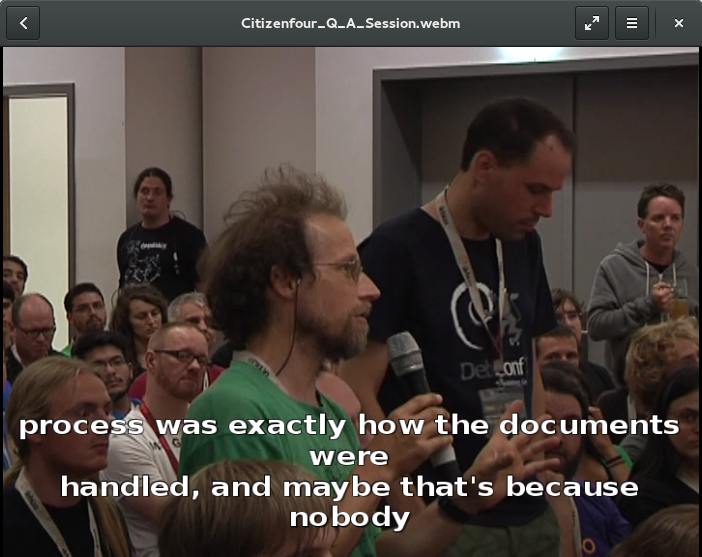
\includegraphics[width=0.8\hsize]{image201510/subtitle.png}
\end{center}
\caption{字幕付き再生例}
\end{figure}
\end{frame}

\begin{frame}{今回のビデオ紹介}

   今回、字幕ファイルがあるビデオのビデオを紹介します。

   具体的なセッション名は、
  \begin{itemize}
\item Stretching out for trustworthy reproducible builds
\item Thanks for maintaining a desktop environment. But is it accessible?
\item Citizenfour Screening
  \end{itemize}

\end{frame}

\begin{frame}{Stretching out for trustworthy(略)}

  タイトルが非常に長い\footnote{まるでライトノベルのタイトル並に長い...}ので略しました。

\begin{figure}[H]
\begin{center}
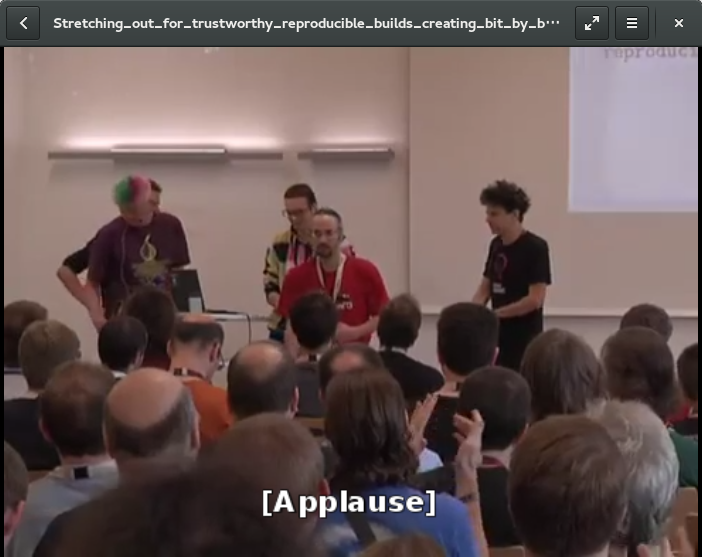
\includegraphics[width=0.8\hsize]{image201510/reproduct.png}
\end{center}
\caption{Stretching out for trustworthy(略)の発表}
\end{figure}
\end{frame}

\begin{frame}{Stretching out for trustworthy(略)つづき}

  ドイツの有名なChaos Computer Club\footnote{Wikipedia-jpで引いてみて下さい。ドイツの有名なコンピュータ技術のエキスパート集団。}にも所属されているDebian開発者らによる、Reproducible Buildsについてのセッションです。

  ビデオ中の目立った話を次頁以降にあげてみます。
\end{frame}

\begin{frame}{Stretching out for trustworthy(略)ハイライト}

  背景説明:
 \begin{itemize}
 \item The 31st Chaos Communication Congress (31C3)\footnote{Chaos Computer Club主催の毎年行われるイベント}にて、パッケージのバイナリにトロイの木馬が巧妙に仕掛けられているか?を調べるにはReproducible Buildsをしたほうが良いという発表を行った。
 \end{itemize}
\end{frame}

\begin{frame}{Stretching out for trustworthy(略)ハイライト}   

  背景説明(つづき):
 \begin{itemize}
\item 31C3のわずか数カ月後に今度はEdward Snowdenさんにより、CIAのStrawhourseというコード名に関するCIA conference 2012の内部文章がリークされた。内容は、MacOS/iOSのSDKに不当な改造を行い、生成されるバイナリにCIAが利用するためのトロイの木馬を仕掛けるという内容。これにより、Reproducible Buildsが益々急務に。リーク文章↓\\
 https://theintercept.com/document/2015/03/10/strawhorse-attacking-macos-ios-software-development-kit/
 \end{itemize}
\end{frame}

\begin{frame}{Stretching out for trustworthy(略)ハイライト}

 Reproducible Buildsのセキュリティ以外の良い点:
 \begin{itemize}
 \item ビルド環境によらず同じバイナリができる、また、クロスビルドの確認ができるようになる、
 \item Debug packageがいつでも(バイナリ作ったあとでも)作れるとか、
 \item FTBFS\footnote{Fails To Build From Sourceの略}が早くわかるとか、
 \item バージョン上げた時の.debの差分が小さくなるとか、
 \end{itemize}

\end{frame}

\begin{frame}{Stretching out for trustworthy(略)ハイライト}

 Reproducible Builds状況:
 \begin{itemize}
 \item Bitcoin/Tor/Corebootは完了している。
 \item Debian/FreeBSD/NetBSD/OpenWrtは進行中。
 \end{itemize}
\end{frame}

\begin{frame}{Stretching out for trustworthy(略)ハイライト}

 Reproducible Buildsにあたっての工夫と苦労:
\begin{itemize}
\item 環境変数SOURCE\_DATE\_EPOCHに時刻(エポック秒)を指定すると、その時刻でビルドしたようにビルドするように様々なツールを改造しupstreamへ提供し取り込んでもらう。なお、これだけでは足らないパッケージが沢山あったらしく、ビルドの日付が埋め込まれる部分をReproducible Builds出来ないとBTSしたりして対策も多数したらしい。
\item tarにビルド環境の都度のユーザ名、グループ名が混じってしまう件の対策。
\item ファイルシステムとlocale環境変数(LANG,LC\_ALL変数)との違いによるソートの振る舞いの違い、プログラムの出力が異なってしまう件の対策
\end{itemize}

が紹介され、実際には相当に苦労されたようです。

\end{frame}

\begin{frame}{Stretching out for trustworthy(略)ハイライト}

 よく、巷では簡単にReproducible Buildsは、パッケージのセキュリティ確認の為と簡単に紹介されますが、実はDebianを構成する重要なソフトウェア・パッケージの多くに手を加えなければ実現できないという大変な偉業を果たしていたという内容でした。
\begin{center}
\LARGE
 彼らの偉業に拍手!
\end{center}  
\end{frame}

\begin{frame}{Thanks for maintaining a desktop...(略)ハイライト}

\begin{figure}[H]
\begin{center}
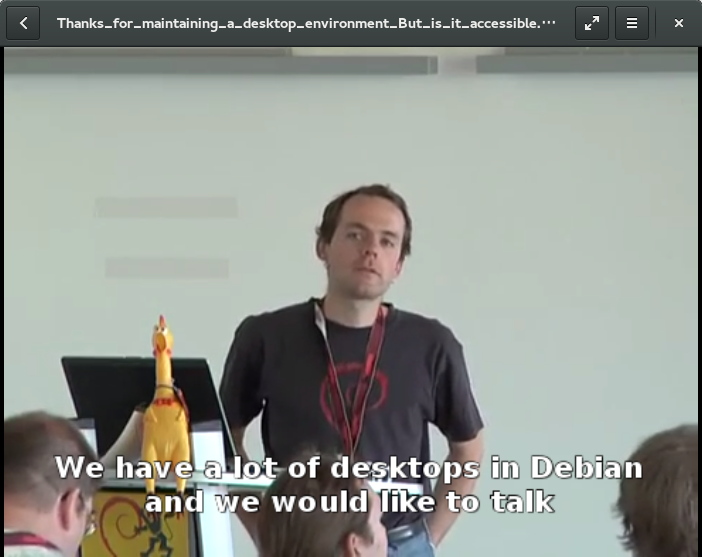
\includegraphics[width=0.5\hsize]{image201510/accessibility.png}
\end{center}
\caption{Thanks for maintaining a desktop...(略)の発表}
\end{figure}

\end{frame}

\begin{frame}{{Thanks for maintaining a desktop...(略)ハイライト}}

  Debian ProjectにてAccessibilityを担当されている方の発表となります。
  Accessibilityに関しての現状と苦労がわかる発表内容。\\
  プレゼン資料↓\\
  http://brl.thefreecat.org/2015-08-22-debconf.pdf

\end{frame}

\begin{frame}{{Thanks for maintaining a desktop...(略)ハイライト}}

   Accessibility留意点:
  \begin{itemize}
\item Free Softwareは、問題があったり、気に入らなかったら、自分で直せるということが基本であるが、Accessibilityの機能を必要としている人は、基本治したくても直せない場合が多いので、コミュニティーによる修正・改善が必須となる。
  \end{itemize}

\end{frame}

\begin{frame}{{Thanks for maintaining a desktop...(略)ハイライト}}

 Linux Desktop環境のAccessibilityの現状:
  \begin{itemize}
  \item Linuxで動作するDesktop環境は、GNOMEがAccessibilityが最もよくできている。
  \item しかしながら、GNOME3を持ってしても、Windowsに比べると10年単位で遅れており、Appleの製品に比べると石器時代の代物と言われても仕方が無い状況。
  \item 弱視の人には、合成音声によるサポートは厳しい場合(そもそも発音しにくいワードの場合など)があるため、理想的には、Piezo braille cellをサポートすべき。
  \end{itemize}

\end{frame}

\begin{frame}{{Thanks for maintaining a desktop...(略)ハイライト}}

 Linux Desktop環境のAccessibilityの現状:
  \begin{itemize}
  \item LinuxのAccessibilityのフレームワーク、
  \item LinuxのAccessibilityのテスト環境など
  \end{itemize}

  は、先述のプレゼン資料を参照ください。Accessibilityがどのようにできていて、どうテストすべきかについて、非常に良い資料となります。
  
\end{frame}

\section{今後のイベント}
\emtext{今後のイベント}
\begin{frame}{今後のイベント}
\begin{itemize}
\item OSC 2015 Tokyo/Fall 10/24出展\&発表。\\
\url{http://www.ospn.jp/osc2015-fall/}
\item 関西エリアDebian勉強会。
\item 11/21(土) 14:00-19:00 第132回東京エリアDebian勉強会
\end{itemize}
\end{frame}

\section{今日の宴会場所}
\emtext{今日の宴会場所}
\begin{frame}{今日の宴会場所}
未定
\end{frame}

\end{document}

;;; Local Variables: ***
;;; outline-regexp: "\\([ 	]*\\\\\\(documentstyle\\|documentclass\\|emtext\\|section\\|begin{frame}\\)\\*?[ 	]*[[{]\\|[]+\\)" ***
;;; End: ***
